%
\section{The Fundamental Data Structures within SpatialDomains}
\label{sec:spatialdomains-datastructures}

As mentioned earlier, in almost all object-oriented languages (which includes $C++$), there exists the concepts of {\em class attributes} and {\em object attributes}.   For a summary of attributes and access patterns, please review Section \ref{sec:stdregions-datastructures}.
Within the SpatialDomains directory of the library, there exists a class inheritance hierarchy designed to try to encourage re-use of core
algorithms (while simultaneously trying to minimize duplication of code).  We present this class hierarchy in Figure \ref{spatialdomains:geomtree}.


\begin{figure}[htb]
\centering
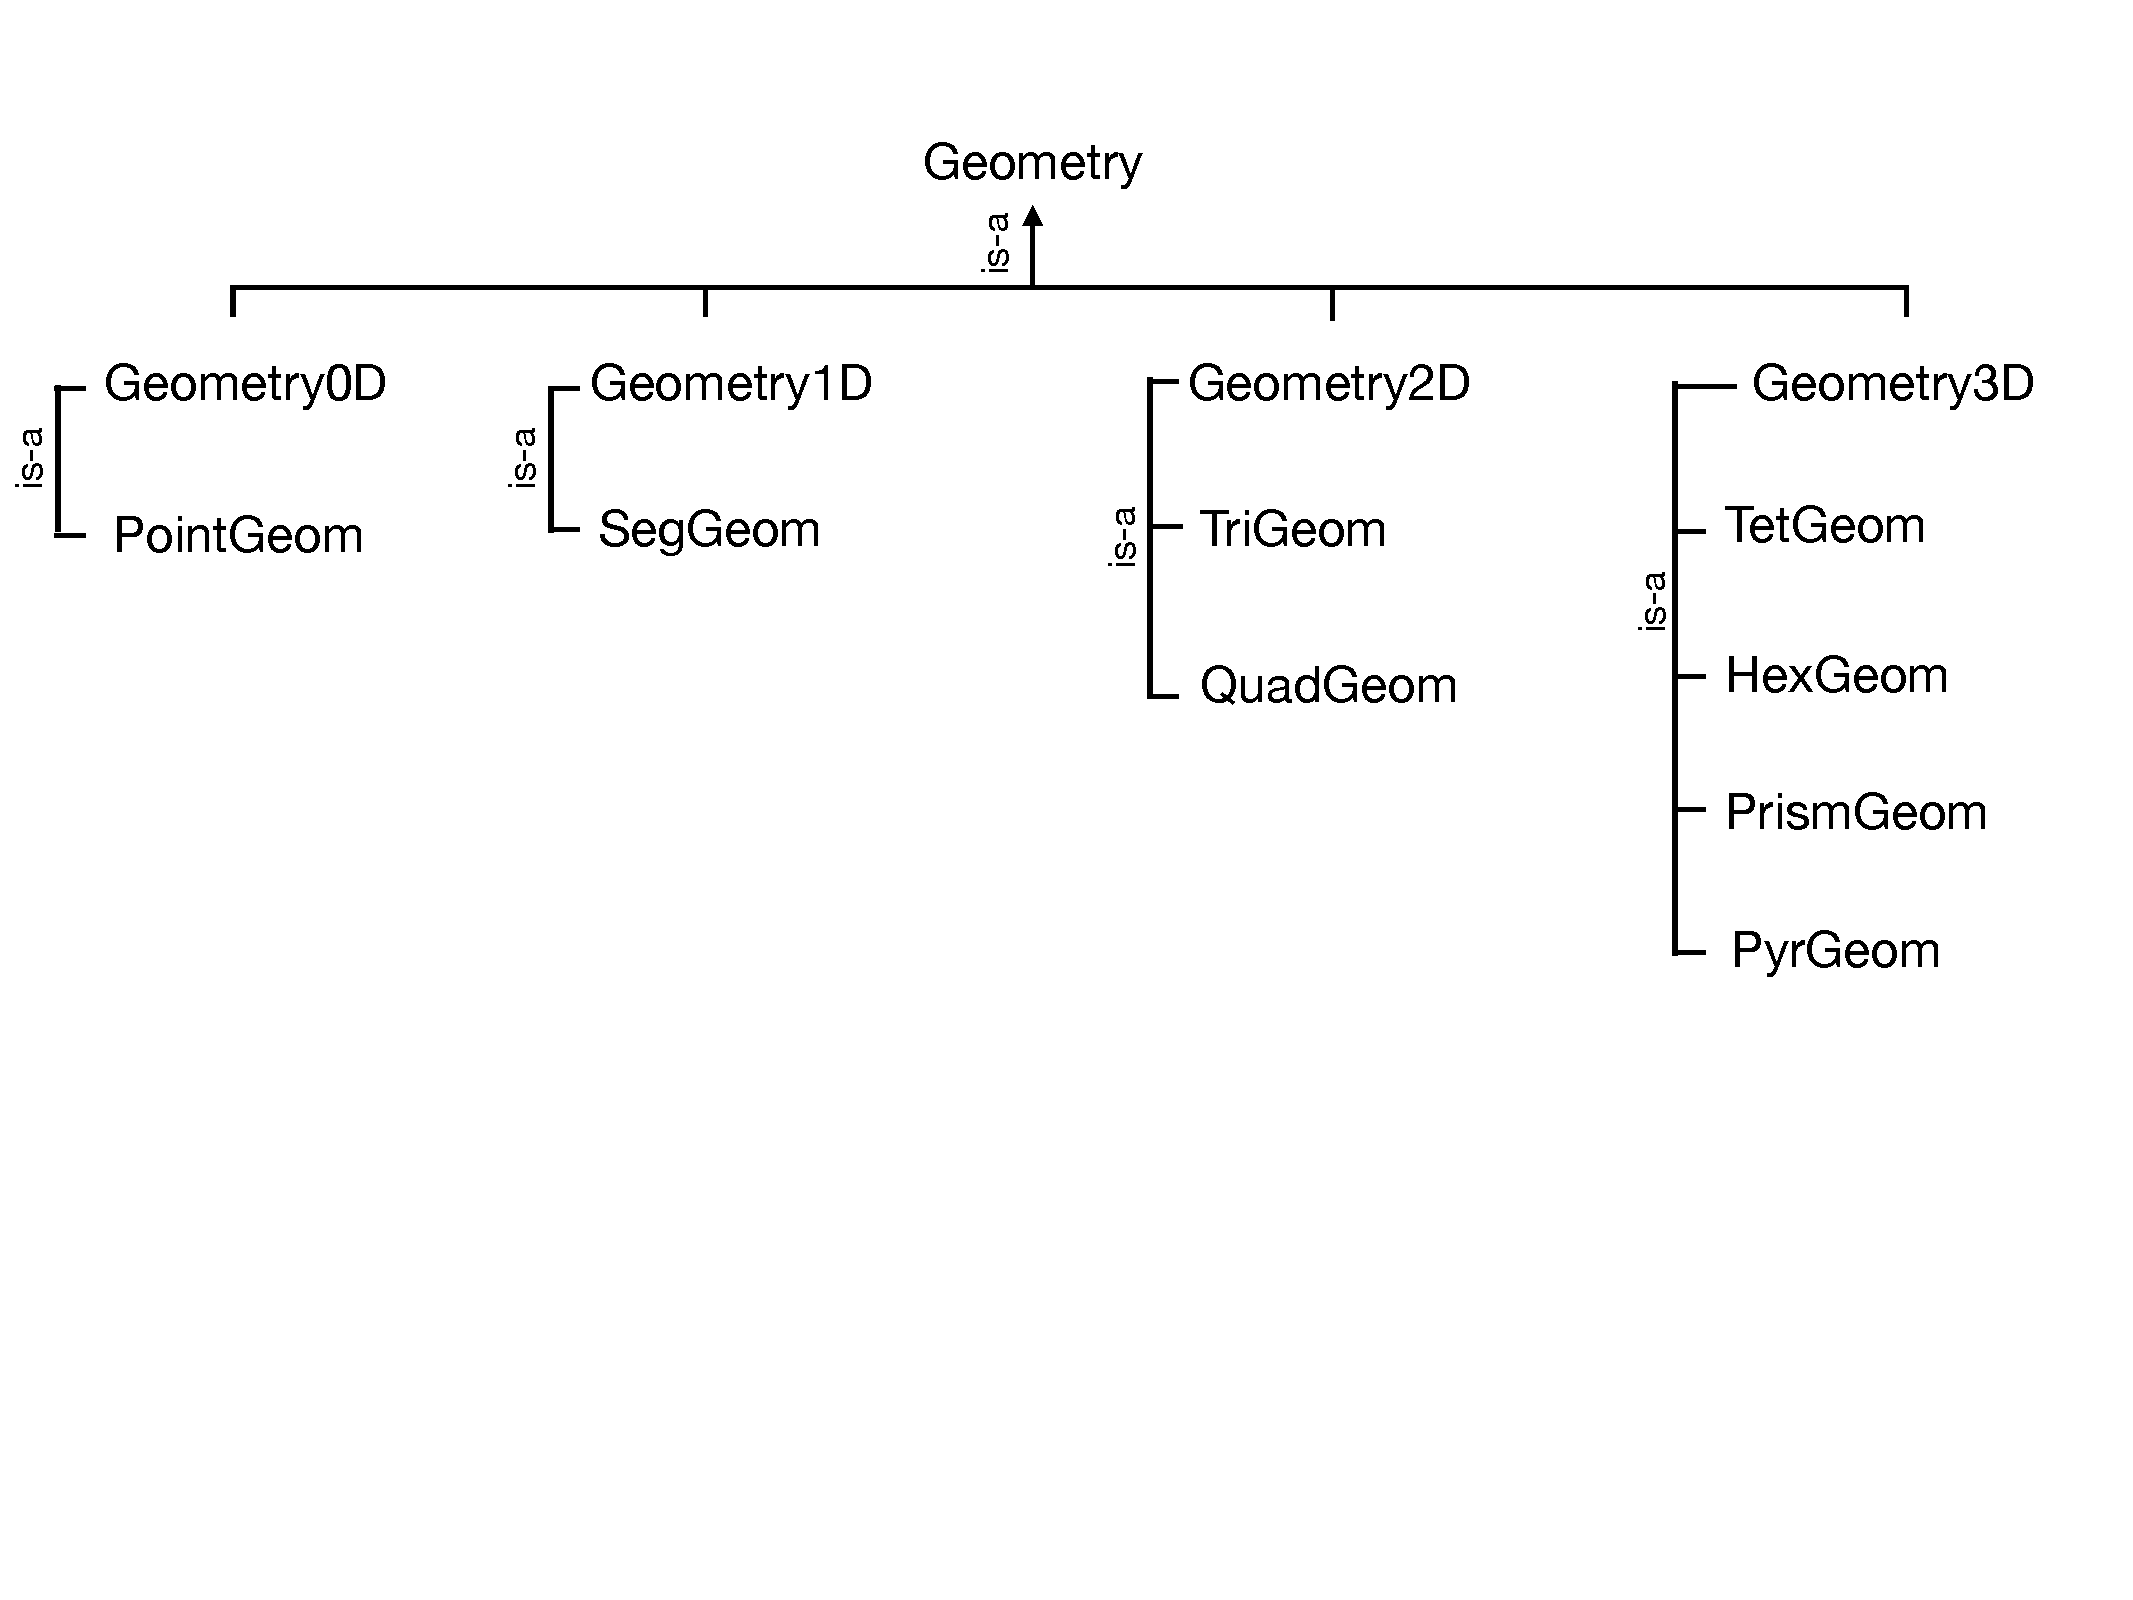
\includegraphics[width=6in]{img/geomtree.pdf}
\caption{Class hierarchy derived from Geometry, the base class of the SpatialDomains Directory.}
\label{spatialdomains:geomtree}
\end{figure}

At its core, the items contained within SpatialDomains are meant to represent the mapping of StdRegion information into world-space.  The various attributes contained herein related to this geometric (mesh, curvature and mapping) information.  The various private, protected and public data members contained within StdRegions are provided in the subsequent sections.


%%%%%%%%%%%%%%%%%%%%%%%%%%%%%%%%%%%%%%%%
\subsection{Variables at the Level of Geometry}

\paragraph{Private:}

\paragraph{Protected:}

\paragraph{Public:}


%%%%%%%%%%%%%%%%%%%%%%%%%%%%%%%%%%%%%%%%
\subsection{Variables at the Level of Geometry\$D for various Dimensions}

\paragraph{Private:}

\paragraph{Protected:}

\paragraph{Public:}

%%%%%%%%%%%%%%%%%%%%%%%%%%%%%%%%%%%%%%%%
\subsection{Variables at the Level of Shape-Specific Geometry Information}

\paragraph{Private:}

\paragraph{Protected:}

\paragraph{Public:}



%%%%%%%%%%%%%%%%%%%%%%%%%%%%%%%%%%%%%
\subsection{Reference to World-Space Mapping}

%%%%%%%%%%%%%%%%%%%%%%%%%%%%%%%%%%%%%
\subsubsection{Geometry}


%%%%%%%%%%%%%%%%%%%%%%%%%%%%%%%%%%%%%
\subsubsection{GeomFactors}




%%%%%%%%%%%%%%%%%%%%%%%%%%%%%%%%%%%%%
\subsection{MeshGraph}